\chapter{Translation in Scratch}

\section{Text to speech and translate}
Scratch 3 the gift that keeps on giving; including the new extensions are Text to Speech and Translate; Text to speech - does as the name suggests, turns typed in phrases into speech via Amazon Web Services. Translate using Google (and I assume Google Translate?) to translate text between different languages.

\begin{figure}
    \centering
    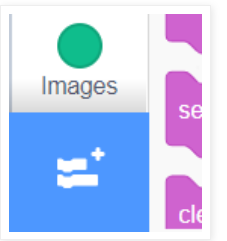
\includegraphics[width=5cm]{chapters/chapterCT1/figures/translat1.png}
    \caption{Extensions button}
    \label{fig:Scratch_extension_button}
\end{figure}

\begin{figure}
    \centering
    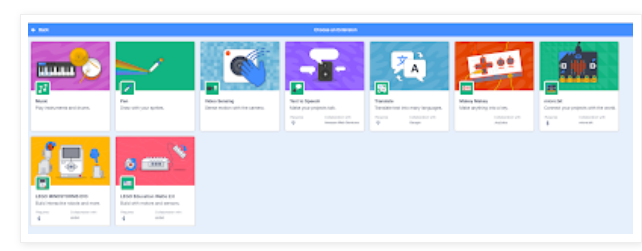
\includegraphics[width=7cm]{chapters/chapterCT1/figures/translate7.png}
    \caption{Scratch_extensions}
    \label{fig:mextensions_l}
\end{figure}


As an experiment, I wanted to  have Scratch the Cat ask me to enter a phrase and then convert that into French, German and Spanish with different voices. The resulting code is shown below.

\begin{figure}
    \centering
    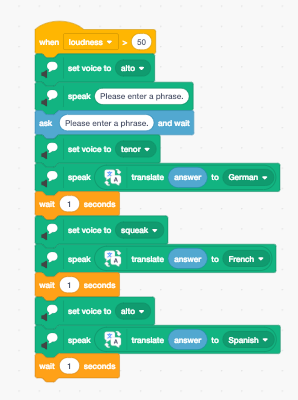
\includegraphics{chapters/chapterCT1/figures/translate8.png}
    \caption{Scratch code to translate}
    \label{fig:scratch_trnslate}
\end{figure}


It is all started by a loud noise like a hand clap. The two extensions have been added to the blocks and are ready to go. The voice is initially set to Alto and the text-speech block has had the phrase "Please enter a phrase" typed in and says this. The ask block has the same question permanently set and the answer produced gets feed into the translations. 

The remaining blocks do essentially the same thing
- change the voice;
- take the phrase typed in (via answer) and convert to the language of choice;
- wait a second.


It is great fun, I am not sure all the languages work but what is there is cool to play with. In an ideal world instead of typing the phrase it would be great to just say the phrase...maybe in the future. 

The code is available at https://scratch.mit.edu/projects/282312832/.
originally published in \url{https://robotsandphysicalcomputing.blogspot.com/2019/01/scratch-speaking-german-french-spanish.html}

\section{speech recognition}
originally published in \url{https://robotsandphysicalcomputing.blogspot.com/2020/07/speech-recognition-turning-hello-into.html}

The Raspberry Pi Foundation recently released a programming activity Alien Language, with support Dale from Machine Learning for Kids, that is a brilliant use of Scratch 3 - Speech Recognition to control a sprite in an alien language. Do the activity, and it is very much worth doing, and it will make sense! I  would also recommend going to the machinelearningforkids.co.uk site anyway it is full of exciting things to do (for example loads of activities https://machinelearningforkids.co.uk/#!/worksheets ). Scratch 3 has lots of extensions that are accessible through the Extension button in the Scratch 3 editor (see below) which add new fun new blocks to play with.




The critical thing for this post is Machine Learning for Kids have created a Scratch 3 template with their own extensions for Scratch 3 within it https://machinelearningforkids.co.uk/scratch3/. One of which is a Speech to Text extension (see below). You must use this one not the standard Scratch 3.

\begin{figure}
    \centering
    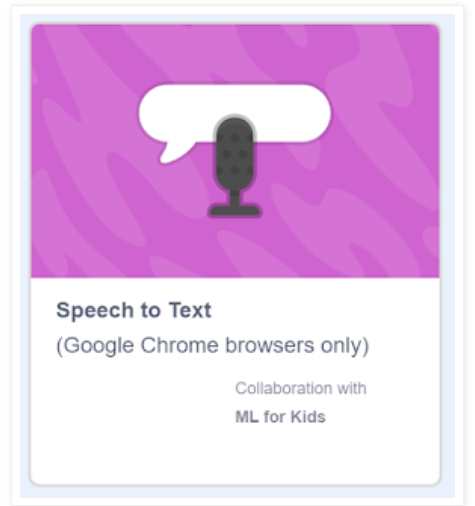
\includegraphics[width=7cm]{chapters/chapterCT1/figures/translate2.png}
    \caption{Speech to Text extension}
    \label{fig:speech to text}
\end{figure}


My idea is to can I set it to react one way when I say "hello"; then say "french" and then say "hello" it says "Bonjour". Two other extensions are needed along with the Speech to Text one - one for speech to text and the translate shown below.

\begin{figure}
    \centering
    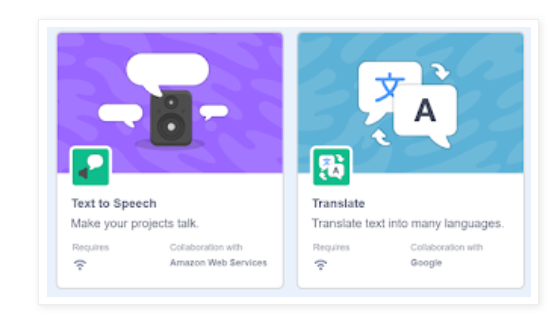
\includegraphics[width=7cm]{chapters/chapterCT1/figures/translate3.png}
    \caption{Other extensions}
    \label{fig:other_extensions}
\end{figure}


Ok, so to the fun bit. The listen and wait, and when I hear blocks are the key new blocks, and they do what they say. The three sets of the code are ones I used for this activity.

\begin{figure}
    \centering
    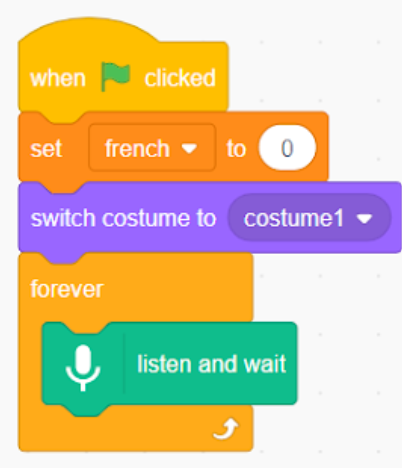
\includegraphics[width=6cm]{chapters/chapterCT1/figures/translate4.png}
    \caption{code 1}
    \label{fig:code1}
\end{figure}
\begin{figure}
    \centering
    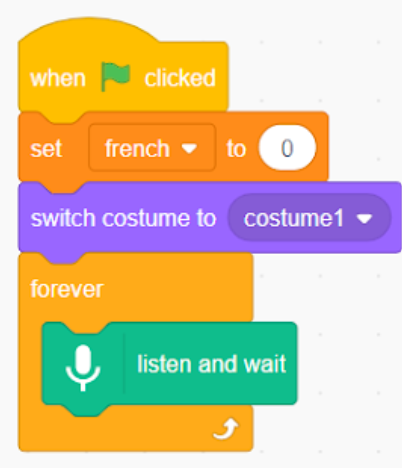
\includegraphics[width=6cm]{chapters/chapterCT1/figures/translate5.png}
    \caption{Code2}
    \label{fig:code2}
\end{figure}
\begin{figure}
    \centering
    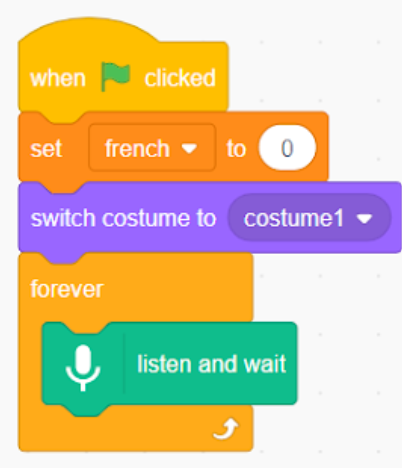
\includegraphics[width=6cm]{chapters/chapterCT1/figures/translate6.png}
    \caption{Code3}
    \label{fig:code3}
\end{figure}



Thank you to Machine Learning for Kids for creating such a brilliant Scratch extension - this is well worth a play with.

